\chapter{Design and Implementation}
\label{implementation}
Our proposed solution of Graphy is implemented into a working prototype running on iOS and Android devices which are backed up by a Unix-like server. In this section, some important features of Graphy as well as the implementation of those features are described.
\section{System Architecture}
As shown in Figure \ref{fg:architecture}, the system contains 2 components: the mobile client and the backend server. The mobile client is an application which interacts directly with a user to capture his/her information. The backend server provides synchronization between multiple clients. Moreover, the backend server can perform additional processing like mining users' data, integrating with other services in the future. The communication between the client and the server is accomplished using the RESTful architecture on top of HTTP/HTTPS protocols.

\begin{figure}[!h]
\begin{centering}
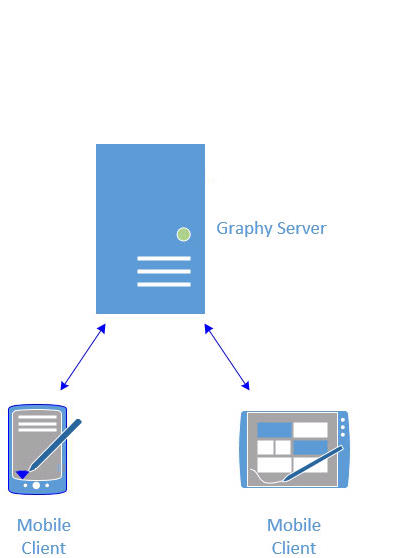
\includegraphics[scale=0.6]{pics/architecture}
\caption{System Architecture}\label{fg:architecture}
\end{centering}
\end{figure}

\section{Mobile Client}
\subsection{Technologies}
The goal of the mobile client is being a fully functional contacts management application. It should provide all nescessary features of a modern Contacts app as well as additional functionalities of Graphy. Moreover, it should run smoothly on popular smart phones. All things considered, we choose to use Xamarin - a state-of-the-art technology which make it possible to do iOS and Android development in C\#. The important thing is that Xamarin allows us to re-use and share a significant amount of code across the two device platforms. Compared with other cross-platform technologies like Sencha or Phonegap, Xamarin have many advantages namely:

\begin{itemize}
\item Native Performance: Xamarin code is compiled so it can leverage platform-specific hardware acceleration.
\item Native User Interfaces: Xamarin utilizes the standard, native user interface elements so apps have different look-and-feel suitable for each platform.
\item Native API Access: Xamarin can access all the functionalities provided by the underlying platform and divice, including platform-specific capabilities.
\end{itemize}

Additionally, the new Xamarin.Forms technology allows us to use the Model-view-viewmodel architectural pattern and share nearly 100\% code on both platforms. The Model-view-viewmodel pattern is our preferred way of separating the graphical user interface and the business logic. Its two-way data bindings automatically synchronize data between controls and models which is very suitable for our application. The architectures of Xamarin and the Model-view-viewmodel pattern can be found in \autoref{fg:xamarin} and \autoref{fg:mvvm_pattern}.

\begin{figure}[!h]
\begin{centering}
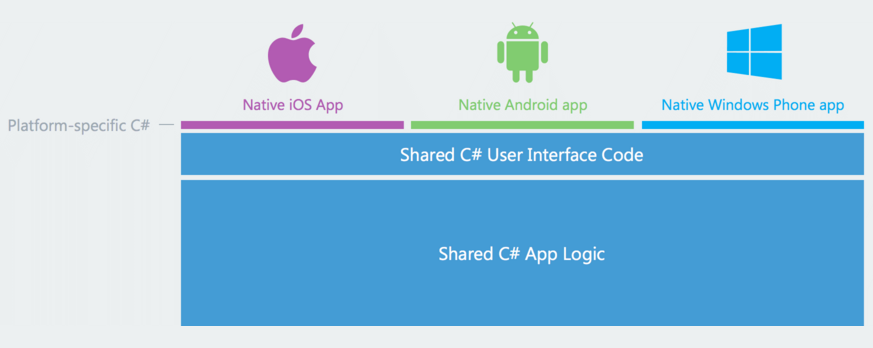
\includegraphics[scale=0.55]{pics/xamarin.png}
\caption{Xamarin Architecture}\label{fg:xamarin}
\source{Reprinted from Xamarin.com, 2016, Retrieved from \textit{www.xamarin.com/platform}}
\end{centering}
\end{figure}

\begin{figure}[!h]
\begin{centering}
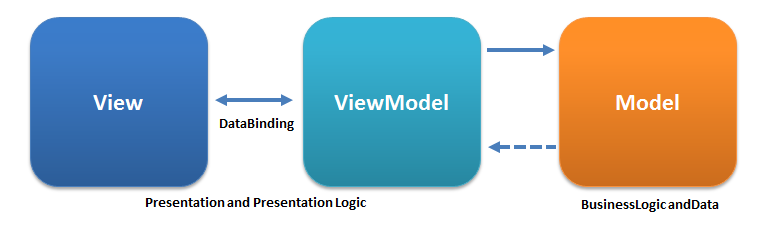
\includegraphics[scale=0.55]{pics/mvvm_pattern.png}
\caption{Model-view-viewmodel Pattern}\label{fg:mvvm_pattern}
\source{Reprinted from Wikipedia.org, 2016, Retrieved from \textit{en.wikipedia.org/wiki/Model-view-viewmodel}}
\end{centering}
\end{figure}

\subsection{Features}
The mobile client has all normal features from a modern contacts management application such as adding/editting/removing contacts, searching for contacts, marking contacts as favorite. Additionally, to make the transition from users' old Contacts application to Graphy effortless, we import all contacts in their phone to Graphy the first time they run our app.

\begin{figure}[!h]\textsl{}
\begin{centering}
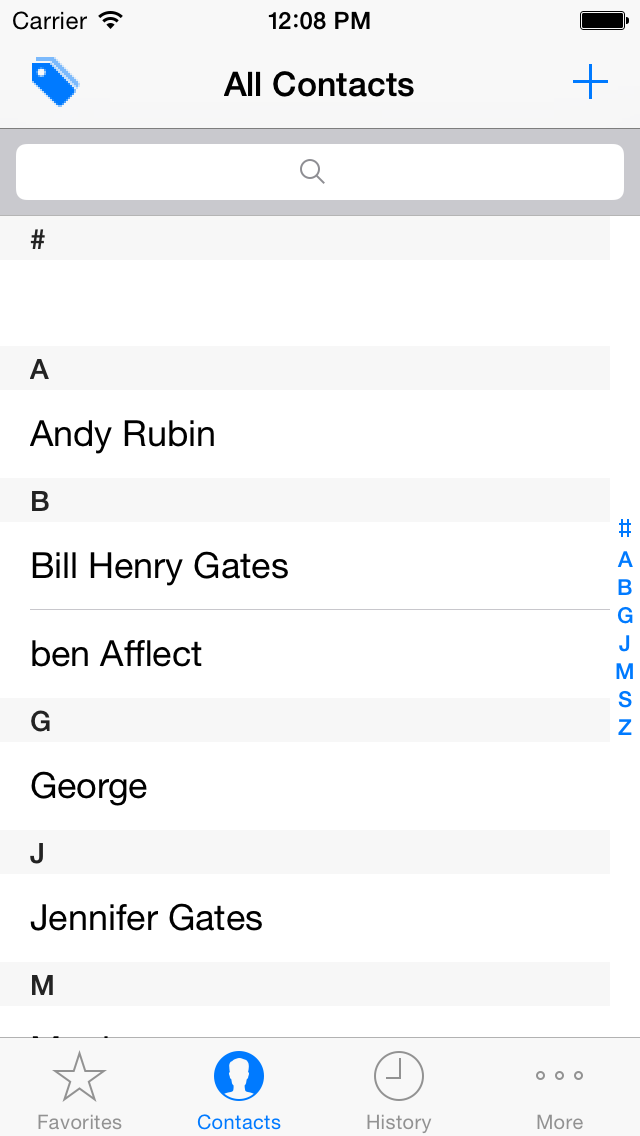
\includegraphics[scale=0.3]{pics/mainscreen}
\caption{Main Screen}\label{fg:mainscreen}
\end{centering}
\end{figure}

More importantly, the feature that distinguishes Graphy from other Contacts applications lies on the contact profiles. As we can see from Figure \ref{fg:contactscreen}, a Graphy's contact profile consists of usual information plus the tags and the relationships. In this example, ``Chairman of Microsoft'' is a custom tag added by the user. The custom tags are implemented by 255-character text fields that cover most common use cases, and users can create as many tags as they want. Furthermore, when a new contact is created, the date and the current location are automatically added as tags in the new contact's profile. These are two historical contexts which may help the user recalling information about the new contact when he/she looks it up again in the future. In later versions, we will add more meaningful historical context tags to assist users better. Regarding relationships between contacts, in Graphy's contact profile, a relationship is demonstrated by 3 fields: the name of the relationship, the related person, and an optional detail about the relationship. In Figure \ref{fg:contactscreen}, Bill Henry Gates is the advisor of Satya Nandela. This relationship is shown by the ``=>'' symbol. Conversely, Jennifer Gates is the daughter of Bill Henry Gates so the symbol is reversed to ``<=''. These symbols are not the most attractive way to represent the relationships and we will design a better user interface in later prototypes. It is worth mentioning that the relationships are bi-directional. When the users tap on the relationships field, Graphy will bring them to the other contact. For example, tapping on Satya Nandela will display the full contact profile of Satya in which there is a relationship ``Advisor'' from Bill Henry Gates. Users can tap infinitely to navigate and explore their relationship networks. Besides, all fields of a relationship are customizable.

\begin{figure}[!h]
\begin{centering}
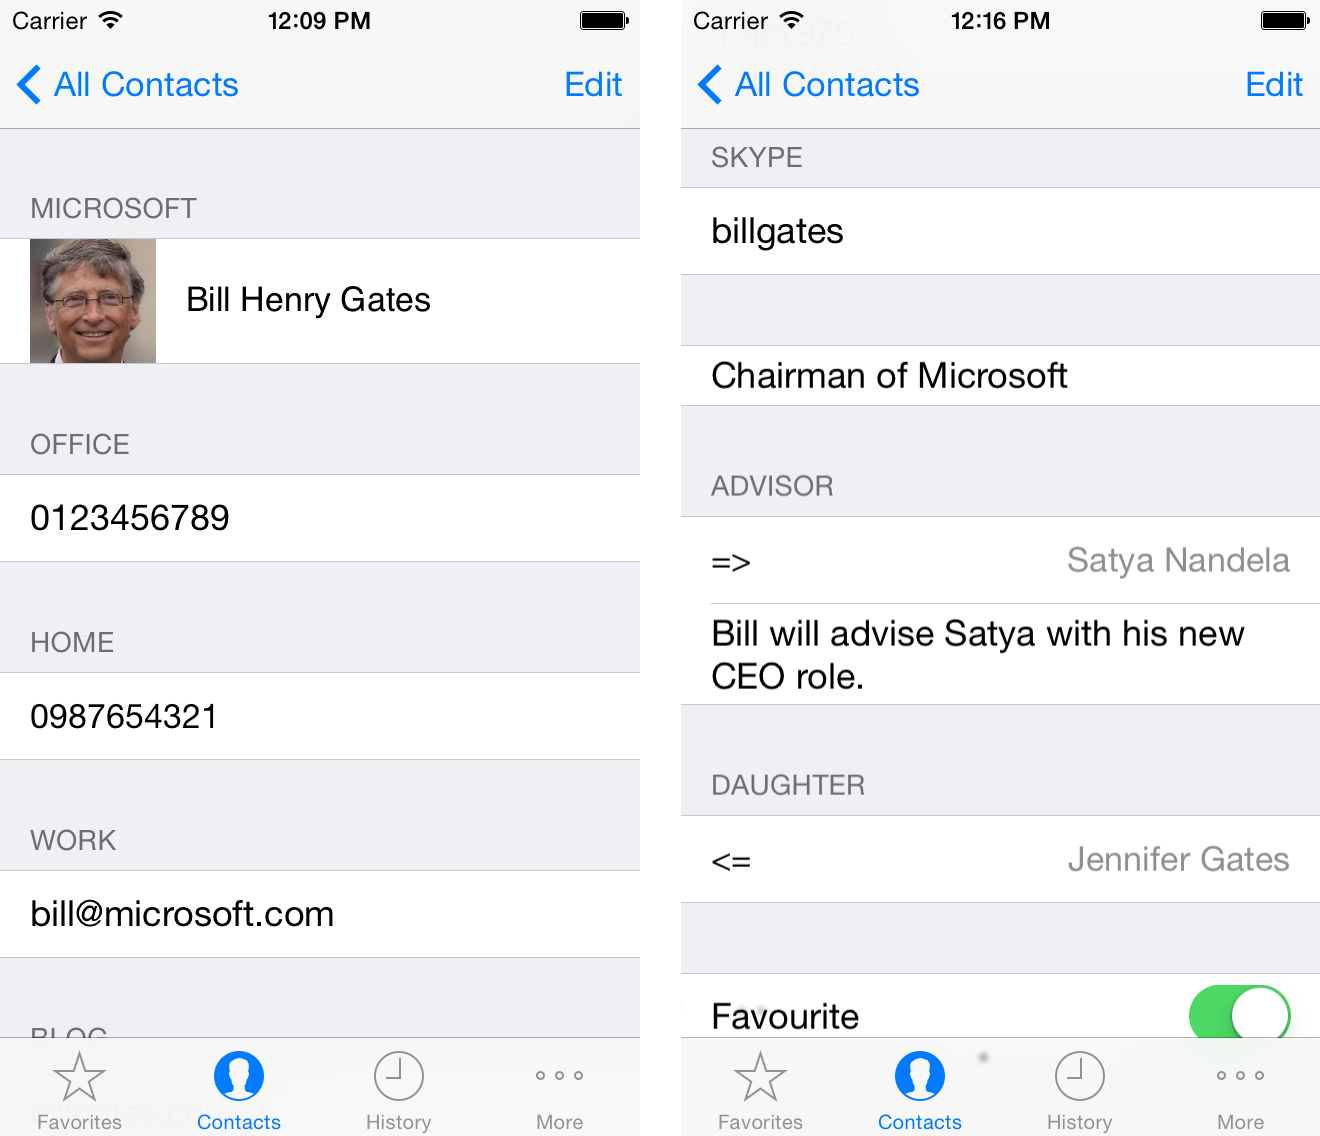
\includegraphics[scale=0.3]{pics/contactscreen}
\caption{Contact Profile}\label{fg:contactscreen}
\end{centering}
\end{figure}

\begin{figure}[!h]
\begin{centering}
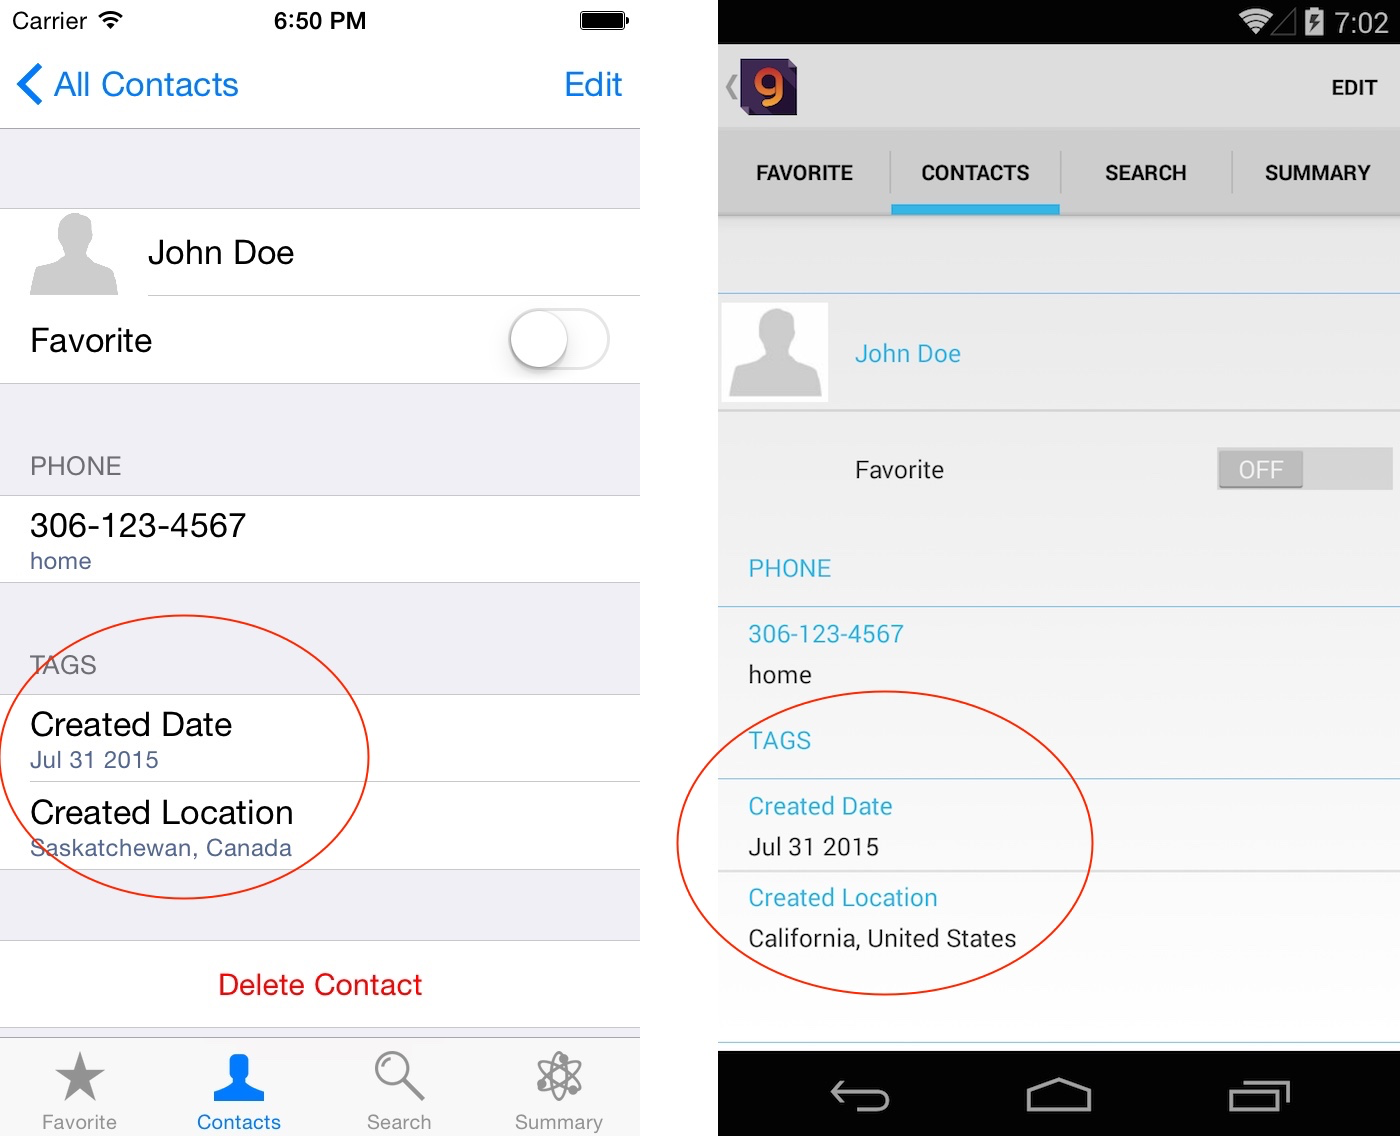
\includegraphics[scale=0.3]{pics/graphy_auto_tag.png}
\caption{Historical Context Tags}\label{fg:/graphy_auto_tag}
\end{centering}
\end{figure}

In addition to the new elements in the contact profiles, we also introduces new ingredients to the search function of the mobile client. Graphy is not only capable of searching for contacts via traditional information like names, organizations but it also supports searching by tags and relationships. Users can enter keywords to Graphy's search boxes then the application will look for that pieces of information in traditional fields, tags, and relationships of all the contacts. Likewise, users can utilize the ``relationships tapping'' feature to jump between contacts and find the people they are looking for. 

The mobile client is fully functional in the offline mode thanks to the implementation of a local SQLite database. When the client connects to the backend server it can synchronize its local database with the server. This design provides the users with the ability to use multiple devices concurrently.

\section{Backend Server}
The goals of the backend server are providing a synchronization service for users on multiple devices, and being a foundation infrastructure for future calculation tasks. One important requirement for the backend server is that it should communicate with the mobile clients through a common and simple protocol. Given these points, we choose HTTP as the protocol, Python as the programing language, Django as the web framework. The Hypertext Transfer Protocol or HTTP is an application protocol for distributed, collaborative, hypermedia information systems \cite{leach1999hypertext}. It is widely used and is the foundation of the World Wide Web's data communication. HTTP operates as a request-response protocol in the client-server computing model. Coupled with HTTP, the Representational state transfer or REST is a state-of-the-art architectural style for designing networked applications. REST can use HTTP for all of its operations. It is a lightweight alternative to Remote Procedure Call and other webservices. In spite of its simplicity, REST is very robust and there is basically nothing we can do in a webservice that cannot be done with REST. Therefore, using REST with the HTTP protocol becomes an excellent choice for our system's communication. Table \ref{tb:restapi} illustrates some example requests of the RESTful API which are exposed by the server. On the other hand, Python is our language of choice since we are familiar with it and it is a powerful, general-purpose programing language. Moreover, the Django web framework, which is written in Python, is an extremely popular open-source framework. It encourages rapid development and clean, pragmatic design while also being fast, secure, and scalable. Django helps us taking care of many aspects in building a RESTful API so we can focusing on the logic of the system. As regards the server, we decide to use a Unix-like local system to run the Gunicorn HTTP server which in turn hosts the Django framework. We prefer this solution instead of using a platform-as-a-service cloud system like Google App Engine or Microsoft Azure because we will have full control of the server and we can avoid some unnecessary cost during the development phase. Later we can rent a server instance from a infrastructure-as-a-service provider like Amazon EC2 to host our system on cloud.

\begin{table}[!ht]
\centering
\caption{RESTful API}\label{tb:restapi}
\begin{tabular}{| l | l | p{3.5cm} |} \hline
\textbf{Verb} & \textbf{Request} & \textbf{Description}\\ \hline
GET & /contacts/ & Retrieve all contacts\\ \hline
POST & /contacts/ & Create a new contact\\ \hline
GET & /contacts/\{id\} & Retrieve a contact with a specific Id\\ \hline
PUT & /contacts/\{id\} & Update a contact\\ \hline
DELETE & /contacts/\{id\} & Delete a contact\\ \hline
\end{tabular}
\end{table}

\section{Database Design and Synchronization}
The databases play an important role in the system of Graphy. Since Graphy operates in both online and offline modes, the local database in a mobile client must contain all user's data. Furthermore, Graphy supports multiple devices concurrently so the databases on clients should synchronize flawlessly and efficiently.

\subsection{Database Schema Design to Support Tagging}\label{databasedesign}
The problem of tagging items has been around in industrial products for a while. It was popularized by websites associated with Web 2.0 and is an important feature of many Web 2.0 services. In 2003, Delicious - a social bookmarking website provided a service for its users to add tags to their bookmarks as a way to help find them later \cite{delicious}. Flickr \cite{flickr} also let users tag their photos with custom information, thus constructing flexible and easy metadata that enriched photos' information and made them highly searchable at the same time. Influenced by the success of Flickr and Delicious' popularized concept, many websites like Youtube \cite{youtube}, Gmail \cite{gmail}, StackOverFlow \cite{stackoverflow} also implemented tagging. Furthermore, the widespread microblogging service Twitter \cite{twitter} introduced the hashtags which let its users tag their own ``tweet'' easily by prefixing the tagged words with a hash symbol. The idea became widely popular and as a result Twitter became a powerful search engine for searching trends or news all over the world. Not only online web services used tags, the operating system OS X version 10.9 also provided colorful tagging labels \cite{osxtag} that helps users to tag their own files.

In order to provide a powerful tagging system (relationship is considered a special type of tag), we need an appropriate database schema. From the database point of view, the tagging problem can be defined as follow: we want to have a database schema where we can tag an item with as many tags as we want. Later on, we want to run queries to constrain the items to a union or intersection of tags. We also want to exclude\slash minus some tags from the search result \cite{puitag}. There are three popular different solutions with which we will examine as follows:

\subsubsection{MySQLicious Solution}
MySQLicious is a library which provides automated mirroring/backups of Delicious bookmarks into a MySQL database \cite{mysqlicious}. The schema of MySQLicious has only one table as shown in Table \ref{tb:mysqlicious}

\begin{table}[!ht]
\centering
\caption{MySQLicious Schema}\label{tb:mysqlicious}
\begin{tabular}{| l | p{5cm} | p{2cm} |} \hline
id & url & tags\\ \hline
1 & \url{http://www.ics.uci.edu/~fielding/pubs} & api\newline rest \newline research \\ \hline
2 & \url{http://stackoverflow.com/questions/983030} & coding\newline .net\\ \hline
3 & \url{http://www.ford.com/cars/mustang/} & cars\newline wishlist\\ \hline
\end{tabular}
\end{table}

In this schema, the table is denormalized. The retrieving queries that can be apply on this schema are as follows:

\textbf{Intersection}\newline
\textit{Query for ``webservices+rest+coding'':}\newline\newline
SELECT *\newline
FROM `MyTable'\newline
WHERE tags LIKE ``\%webservice\%''\newline
AND tags LIKE ``\%rest\%''\newline
AND tags LIKE ``\%coding\%''

\textbf{Union}\newline
\textit{Query for ``webservices|rest|coding'':}\newline\newline
SELECT *\newline
FROM `MyTable'\newline
WHERE tags LIKE ``\%webservice\%''\newline
OR tags LIKE ``\%rest\%''\newline
OR tags LIKE ``\%coding\%''

\textbf{Minus}\newline
\textit{Query for ``webservices+rest-coding'':}\newline\newline
SELECT *\newline
FROM `MyTable'\newline
WHERE tags LIKE ``\%webservice\%''\newline
AND tags LIKE ``\%rest\%''\newline
AND tags NOT LIKE ``\%coding\%''

The advantages of this solution are:
\begin{itemize}
   \item Just one table.
   \item The retrieving queries are very straight forward.
   \item Can achieve results via full-text search which can be a little faster.
\end{itemize}

The disadvantages are:
\begin{itemize}
   \item We have a limit on the number of tags per item according to the size of the tags field. Normally we use a 256-byte field in our database (VARCHAR). Otherwise, if we use a text field or the like, the queries will become slow.
   \item Doing processing on tags is hard and expensive. For example, it is difficult to provide suggestions on a new tag. Therefore, synonymous tag names like ``coding'' and ``programing'' have a high chance of happening.
\end{itemize}

\subsubsection{Scuttle Solution}
Similar to Delicious, Scuttle \cite{scuttle} is a web-based social bookmarking system. It allows multiple users to store, share and tag their favorite links online. Scuttle organizes its data in two tables as shown in Figure \ref{fg:scuttle}. The table scCategories is the tag-table and has got a foreign key to the bookmark-table.

\begin{figure}[!h]
\begin{centering}
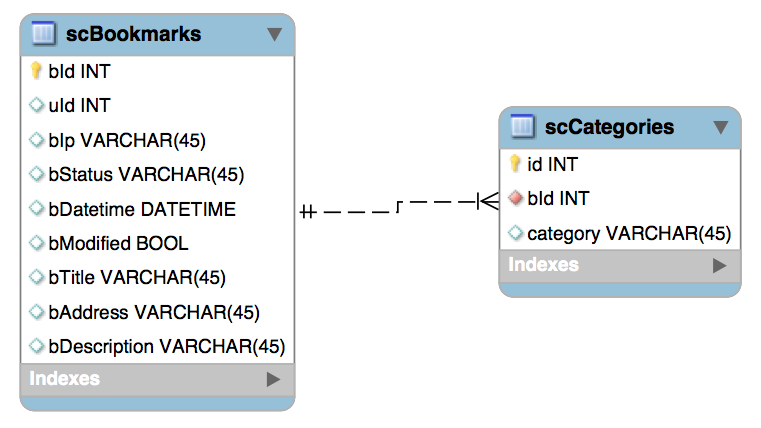
\includegraphics[scale=0.5]{pics/scuttle}
\caption{Scuttle Schema}\label{fg:scuttle}
\end{centering}
\end{figure}

The retrieving queries we can apply on this schema are as follows:

\textbf{Intersection}\newline
\textit{Query for ``webservices+rest+coding'':}\newline\newline
SELECT b.*\newline
FROM `scBookmark' b, `scCategories' c\newline
WHERE b.bId = c.bId\newline
AND (c.category IN (`webservices', `rest', `coding'))\newline
GROUP BY b.bId\newline
HAVING COUNT(b.bId)=3

Firstly, all combinations of bookmarks and tags are searched, where the tag is ``webservices'', ``rest'' or ``coding'' (c.category IN (`webservices', `rest', `coding')), then just the bookmarks that have all three tags are selected (HAVING COUNT(b.bId)=3).

\textbf{Union}\newline
\textit{Query for ``webservices|rest|coding'':}\newline\newline
SELECT b.*\newline
FROM `scBookmark' b, `scCategories' c\newline
WHERE b.bId = c.bId\newline
AND (c.category IN (`webservices', `rest', `coding'))\newline
GROUP BY b.bId

\textbf{Minus}\newline
\textit{Query for ``webservices+rest-coding'':}\newline\newline
SELECT b.*\newline
FROM `scBookmark' b, `scCategories' c\newline
WHERE b.bId = c.bId\newline
AND (c.category IN (`webservices', `rest'))\newline
AND b.bId NOT\newline
IN (SELECT b.bId FROM scBookmarks b, scCategories c WHERE b.bId = c.bId AND c.category = 'coding')\newline
GROUP BY b.bId\newline
HAVING COUNT(b.bId) =2

The advantages of this solution are:
\begin{itemize}
   \item The schema is more normalized than the MySQLicious solution.
   \item Listing and doing processing on all tags in the system is rather easy.
\end{itemize}

The disadvantages are:
\begin{itemize}
   \item The retrieving queries have JOIN queries which might be more expensive.
   \item There are many duplicated tags in the system since one tag record in the tag-table only associates with one item in the bookmark-table.
\end{itemize}

\subsubsection{Toxi Solution}
Toxi \cite{toxi} an open-source software contributor came up with a three-table schema as shown in Figure \ref{fg:toxi}. The bookmarks and the tags are n-to-m related by making use of a tagmap table. As a result, we can use one tag for many bookmarks and vice versa. This structure is also used by the popular blogging platform WordPress \cite{wordpress}.

\begin{figure}[!h]
\begin{centering}
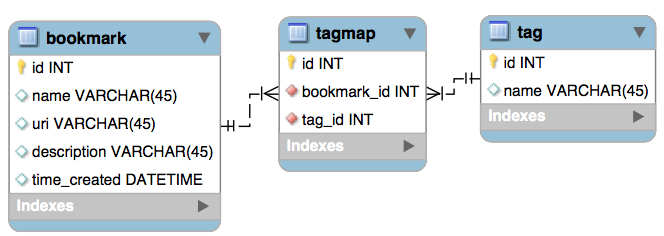
\includegraphics[scale=0.65]{pics/toxi}
\caption{Toxi Schema}\label{fg:toxi}
\end{centering}
\end{figure}

The retrieving queries we can apply on this schema are as follows:

\textbf{Intersection}\newline
\textit{Query for ``webservices+rest+coding'':}\newline\newline
SELECT b.*\newline
FROM tagmap bt, bookmark b, tag t\newline
WHERE bt.tag\_id = t.id\newline
AND (t.name IN (`webservices', `rest', `coding'))\newline
AND b.id = bt.bookmark\_id\newline
GROUP BY b.id\newline
HAVING COUNT(b.id)=3

\textbf{Union}\newline
\textit{Query for ``webservices|rest|coding'':}\newline\newline
SELECT b.*\newline
FROM tagmap bt, bookmark b, tag t\newline
WHERE bt.tag\_id = t.id\newline
AND (t.name IN (`webservices', `rest', `coding'))\newline
AND b.id = bt.bookmark\_id\newline
GROUP BY b.id

\textbf{Minus}\newline
\textit{Query for ``webservices+rest-coding'':}\newline\newline
SELECT b.*\newline
FROM bookmark b, tagmap bt, tag t\newline
WHERE b.id = bt.bookmark\_id\newline
AND (t.name IN (`webservices', `rest'))\newline
% AND b.id NOT\newline % Probably typo
AND b.id NOT IN (SELECT b.id FROM bookmark b, tagmap bt, tag t\newline
WHERE b.id = bt.bookmark\_id AND bt.tag\_id = t.id AND t.name = `coding'\newline
GROUP BY b.id\newline
HAVING COUNT(b.id) =2

The advantages of this solution are:
\begin{itemize}
   \item The schema is in the Third Normal Form. It is the most normalized solution of all three.
   \item We can add extra information to each tag such as description, tag hierarchy. 
   \item Doing processing on tags is easy.
   \item Flexible, scaling well.
\end{itemize}

The disadvantages are:
\begin{itemize}
   \item The retrieving queries are quite expensive and can become very complicated. However, we can break down a complicated query and utilize the cache.
   \item Altering or deleting bookmarks can lead to orphan tag unless we use cascading.
\end{itemize}

\subsubsection{Schema Performance Analysis}
\paragraph{Test Setups}
Eachhome \cite{puiperformance} did performance tests on all the solutions mentioned above: MySQLicious, MySQLicious with full-text search, Scuttle and Toxi. The test setups are as follows:

For each schema, there are 4 databases of 1000, 10000, 100000 and 1 million bookmarks. The tags associated with the bookmarks were random English words. Each bookmark got 1 to 10 tags attached to it. Every schema had exactly the same data. Then each schema was queried with an alternately 1-3 tag query. For example, the first query was ``webservice'', the second was ``webservice+rest'', the third was ``webservice+rest+coding'', the fourth again was just one tag like the first one and so forth. 
Each query was done with LIMIT 50. All the queries worked and the outcomes were the same on all schemas.

The databased was MySQL 4.0.21 with the configuration described in Table \ref{tb:mysqlconfig}.

\begin{table}[!ht]
\centering
\caption{MySQL Configuration}\label{tb:mysqlconfig}
\begin{tabular}{| l |} \hline
key\_buffer = 300M \\ \hline
query\_cache\_size = 30M \\ \hline
query\_cache\_limit = 30M \\ \hline
table\_cache = 64 \\ \hline
ft\_min\_word\_len = 2 \\ \hline
ft\_stopword\_file = `' \\ \hline
\end{tabular}
\end{table}

Detail of the computation system is described in Table \ref{tb:systemconf}.

\begin{table}[!ht]
\centering
\caption{System Configuration}\label{tb:systemconf}
\begin{tabular}{| l | l |} \hline
CPU & 3GHz Dual Xeon\\ \hline
Cache & 1MB\\ \hline
Harddisk & SCSI Ultra 320 Atlas 10K, no RAID\\ \hline
RAM & 3GB\\ \hline
\end{tabular}
\end{table}

\paragraph{Test Results}

The first test was done with a tag set of 250 tags. As we can see from Figure \ref{fg:intersection250}, when  the tag number of items was smaller than 10 thousands, all schemas performed very well. The differences in performance only appeared when the dataset was 1 million or more. When the number of bookmarks was 1 million, MySQLicious was very slow because of the filter instruction \textit{WHERE tag LIKE ``\%tagname\%''}. That was, MySQLicious had to go through the whole dataset to test each item against the queries. Moreover, applying full-text search did not make this solution any faster. On the contrary, Toxi solution was really fast. It was about twice as fast as the Scuttle solution and four times faster than MySQLicious.

\begin{figure}[!h]
\begin{centering}
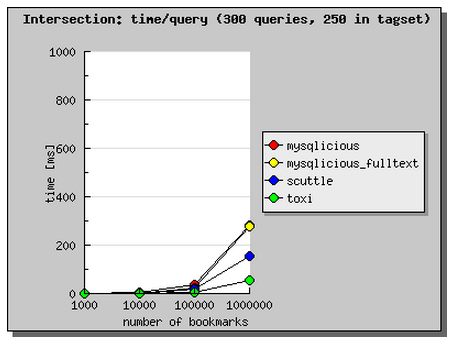
\includegraphics[scale=0.8]{pics/intersection250}
\caption{Intersection Queries with 250 Tag Set}\label{fg:intersection250}
\end{centering}
\end{figure}

The second test was done with a 999 tag set. Looking at what happened in Figure \ref{fg:intersection999}, MySQLicious with full-text search was the performance leader. It indicated that if we have a system with diverse tag distribution, MySQLicious with full-text search will be the best solution. According to Eachhome research \cite{puiperformance}, if a system has an average tag distribution of 1\% (a tag shows up in 1/100 of all items on an average), Toxi is the best solution. On the other hand, if the system is more uniformly ditributed, MySQLicious performs better.

\begin{figure}[!h]
\begin{centering}
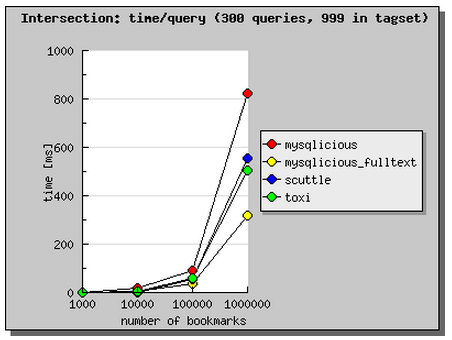
\includegraphics[scale=0.8]{pics/intersection999}
\caption{Intersection Queries with 999 Tag Set}\label{fg:intersection999}
\end{centering}
\end{figure}

Regarding Union queries, MySQLicious was the fastest as we can see in Figure \ref{fg:union250}. Taking advantage of the \textit{LIKE} queries, MySQLicious sought through all the items then harvested the items with one of the given tags. The magic here lay in the \textit{LIMIT} instruction. MySQLicious traversed the items, checked the constraints then stopped after finding enough items as specified in the \textit{LIMIT} instruction. Whereas in other solutions, the database had to join the tags with the items first then searched through the join result, thus increasing a significant amount of time.

\begin{figure}[!h]
\begin{centering}
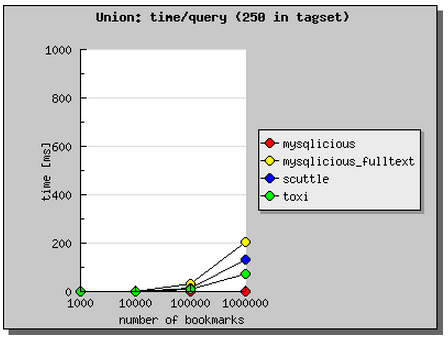
\includegraphics[scale=0.8]{pics/union250}
\caption{Union Queries with 250 Tag Set}\label{fg:union250}
\end{centering}
\end{figure}

Compared with intersection and union queries, insertion queries are remarkably faster. In Figure \ref{fg:insert250}, the scale of the vertical-axis changed to 0 - 2 millisecond. MySQLicious handled insertion queries very well, its variation of full-text had to create the full-text index and therefore was a little slower. The Scuttle and Toxi solutions are slower because of the creation of the second and the third tables in their schema. However, insertion queries in all schemas were still about 100 times faster than intersection and union ones. Therefore, we should base our schema decisions on intersection and union queries. 

\begin{figure}[!h]
\begin{centering}
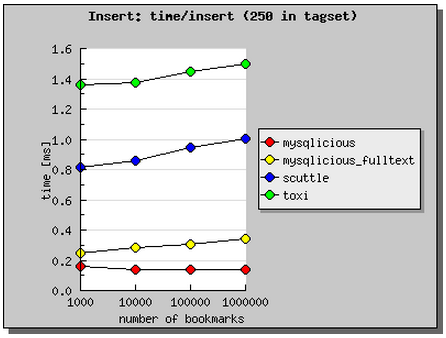
\includegraphics[scale=0.8]{pics/insert250}
\caption{Insertion Queries with 250 Tag Set}\label{fg:insert250}
\end{centering}
\end{figure}

\paragraph{Improving Performance}
There are four popular ways to improve the performance. First, we can use \textit{Caching}, we can cache the results of the recent queries for some hours or cache the items per tag. Second, we can use both MySQLicious full-text and Toxi solutions at the same time then use the appropriate schema based on the characteristic of the queries. For example, simple union queries will be performed on MySQLicious while intersection queries with common tags on Toxi. Third, we can slice the data to user/tag/item and prebuild some results. Forth, we can use a NoSQL database. However, using a NoSQL database will lead to other requirements which need to be taken care of.

\subsubsection{Conclusion}
The nature of a Contact application requires consistency on a small dataset (less than 1 million records). Therefore, we choose the Toxi \cite{toxi} solution which has been discussed above. The local database on a mobile client uses SQLite. It processes all user's queries locally then automatically synchronizes with server database when there is an Internet connection. The server uses a PostgreSQL database with a slight change in the schema to store data from all users. Parts of the database schema are shown in Figure \ref{fg:dbtag} and Figure \ref{fg:dbrelationship}.

\begin{figure}[!h]
\begin{centering}
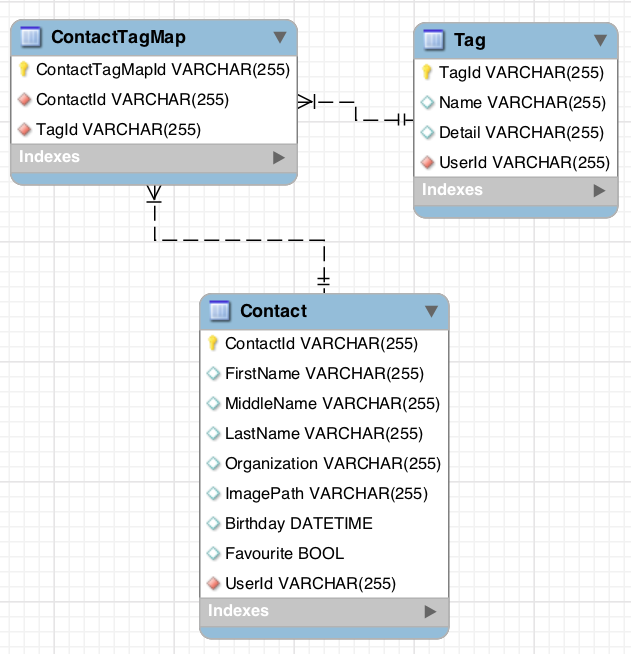
\includegraphics[scale=0.5]{pics/dbtag}
\caption{Tag Schema}\label{fg:dbtag}
\end{centering}
\end{figure}

\begin{figure}[!h]
\begin{centering}
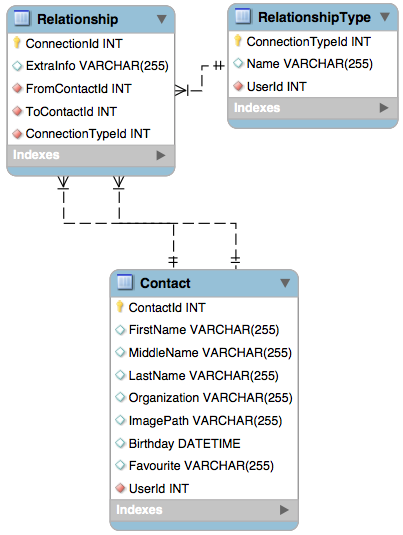
\includegraphics[scale=0.5]{pics/dbrelationship}
\caption{Relationship Schema}\label{fg:dbrelationship}
\end{centering}
\end{figure}

\subsection{Synchronization Technique}
In order to provide an efficient synchronization solution, each Graphy's mobile client maintains a Sync Queue in its local database. When the user creates, updates or deletes a record, the operation will be applied immediately to the local database and at the same time that operation will also be appended to the Sync Queue. When the mobile client has Internet connection, Graphy will periodically communicate with the backend server to sync the current operations in the Sync Queue to the database on server. Since our work is not focusing on designing a synchronization algorithm, we make an assumption that the mobile clients and the backend server are always having the same clock. Obviously, the clock synchronization process can be done by applying a well-known method such as Network Time Protocol, TLSDate, or using versions.

The synchronization process is briefly described as follows:

% Old algorithm!!
%\begin{enumerate}
%   \item Client sends GET requests to all endpoints of the API. The GET requests contain a IF-MODIFIED-SINCE header and a IF-UNMODIFIED-SINCE header. The IF-MODIFIED-SINCE header is set equal to the previous sync time of the client, the IF-UNMODIFIED-SINCE header is set equal to the current sync time which we receive in step 1. After that, client updates its database and sync queue based on the responses received from all requests.
%
%   \item Client consecutively performs all operations in its Sync Queue:
%     \begin{enumerate}
%       \item If the operation is a creation:
%         \begin{enumerate}
%           \item Client sends a POST request to server with detail of the new \textit{local record} in the request's body.
%           \item Server creates a new \textit{server record} according to the request's body and a last\_modified field equal to current time at server.
%           \item Server sends back to client an HTTP 201 CREATED response which contains the \textit{server record}.
%           \item Client updates the \textit{local record's} last\_modified according to the \textit{server record's}.
%         \end{enumerate}
%         
%       \item If the operation is an update:
%         \begin{enumerate}
%           \item Client sends a PUT request to server with details of the updated \textit{local record} in the request's body.
%           \item Server changes the \textit{server record} according to the request's body then updates the last\_modified field with the current time at server.
%           \item Server sends back to client an HTTP 200 OK response which contains the \textit{server record}.
%           \item Client updates the \textit{local record's} last\_modified according to the \textit{server record's} last\_modified field.
%         \end{enumerate}
%               
%       \item If the operation is a deletion:
%         \begin{enumerate}
%           \item Client sends a DELETE request to server with \textit{local record's} last\_modified field in the request's argument.
%           \item If the \textit{local record's} last\_modified field equals the \textit{server record's} one then server sets the lazy delete flag is\_deleted on the \textit{server record} to TRUE. If the last\_modified fields are not equal then the server does nothing.
%           \item Server sends back to client an HTTP 202 ACCEPTED response.
%         \end{enumerate}         
%     \end{enumerate}
%
%   \item Client sets its last sync time to the current sync time received in step 1.
%\end{enumerate}

\begin{enumerate}
   \item Client sends GET requests to all endpoints of the API. The server returns all records of that user. After that, the client examines the server's records, if they have the last\_modified field greater than the client's ones, the client will update its database and Sync Queue according to the information from the server.

   \item Client consecutively performs all operations in its Sync Queue:
     \begin{enumerate}
       \item If the operation is a creation:
         \begin{enumerate}
           \item Client sends a POST request to the server with detail of the new \textit{client record} in the request's body.
           \item Server creates a new \textit{server record} according to the request's body. 
           \item Server sends back to client an HTTP 201 CREATED response which contains the \textit{server record}.
         \end{enumerate}
         
       \item If the operation is an update:
         \begin{enumerate}
           \item Client sends a PUT request to server with details of the updated \textit{client record} in the request's body.
           \item Server examines the \textit{client record}. The server will return one of the three HTTP responses: 204 NO CONTENT, 409 CONFLICT, or 410 GONE after comparing the \textit{client record} and the \textit{server record}. 
           \item Client receives the server response and bases on it to make decision on keeping, updating or deleting the \textit{client record}.
         \end{enumerate}
               
       \item If the operation is a deletion:
         \begin{enumerate}
           \item Client sends a DELETE request to server with the ID of the \textit{client record} and an IF-UNMODIFIED-SINCE header which is set to be equal to the record's last\_modified field.
           \item Server examines the \textit{client record} and compare it with the \textit{server record}. After that, it will decide to mark the \textit{server record} deleted or not, then return one of the three HTTP responses: 204 NO CONTENT, 409 CONFLICT, or 410 GONE.
           \item Client receives the server response and bases on it to make decision on keeping or deleting the \textit{client record}. 
         \end{enumerate}         
     \end{enumerate}
\end{enumerate}
